\documentclass[tikz,border=3pt]{standalone}
\usetikzlibrary{arrows.meta,calc}
\begin{document}
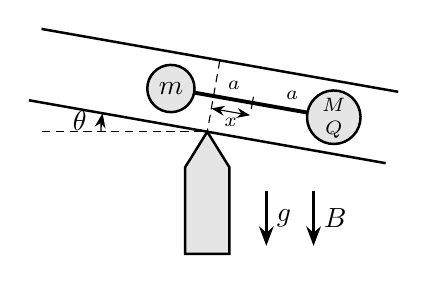
\begin{tikzpicture}[scale=1.0,>=Stealth,line width=0.9pt]
  \def\ang{-10}
  \def\xc{0.50}
  \def\aa{1.05}

  % 支柱（支点を原点 (0,0) とする）
  \draw[fill=black!10] (-0.28,-1.55) -- (-0.28,-0.45) -- (0,0) -- (0.28,-0.45) -- (0.28,-1.55) -- cycle;

  % 水平の基準線（支点の高さに合わせる）
  \draw[line width=0.4pt,densely dashed] (-2.1,0) -- (0,0);

  % 傾いた管と内部の質点・棒（支点と管の底が (0,0) で接する）
  \begin{scope}[rotate around={\ang:(0,0)}]
    \draw (-2.3,0) -- (2.3,0);
    \draw (-2.3,0.92) -- (2.3,0.92);

    \coordinate (Lm) at (\xc-\aa, 0.46);
    \coordinate (Cc) at (\xc, 0.46);
    \coordinate (RM) at (\xc+\aa, 0.46);

    \draw[line width=1.4pt] (Lm) -- (RM);
    \draw[fill=black!10] (Lm) circle (0.30);
    \node at (Lm) {$m$};
    \draw[fill=black!10] (RM) circle (0.34);
    \node[yshift=4.5pt] at (RM) {\scriptsize $M$};
    \node[yshift=-4.5pt] at (RM) {\scriptsize $Q$};

    % 支点の位置と棒の中心の目印
    \draw[line width=0.4pt,densely dashed] (0,0.92) -- (0,0);
    \draw[line width=0.4pt] (\xc,0.54) -- (\xc,0.38);
    \draw[line width=0.4pt,<->] (0,0.30) -- (\xc,0.30);
    \node[below,inner sep=1.5pt] at (0.5*\xc,0.29) {\scriptsize $x$};

    % 長さ a の表示（破線と重ならない位置に配置）
    \node[above,inner sep=1.5pt] at (0.25,0.52) {\scriptsize $a$};
    \node[above,inner sep=1.5pt] at (\xc+0.48*\aa,0.52) {\scriptsize $a$};
  \end{scope}

  % 傾き角 theta の表示（水平破線と管の底の間）
  \draw[line width=0.5pt,->] (-1.35,0) arc[start angle=180,end angle={180+\ang},radius=1.35];
  \node[left] at (-1.40,0.14) {$\theta$};

  % 重力と磁場（鉛直下向き）
  \draw[->] (0.75,-0.75) -- (0.75,-1.45);
  \node[right] at (0.75,-1.10) {$g$};
  \draw[->] (1.35,-0.75) -- (1.35,-1.45);
  \node[right] at (1.35,-1.10) {$B$};
\end{tikzpicture}
\end{document}
